\subsection{Brain Similarity of Large Language Models}

\begin{figure}[!t]
  \centering
  % \fbox{\rule[-.5cm]{0cm}{4cm} \rule[-.5cm]{4cm}{0cm}}
  {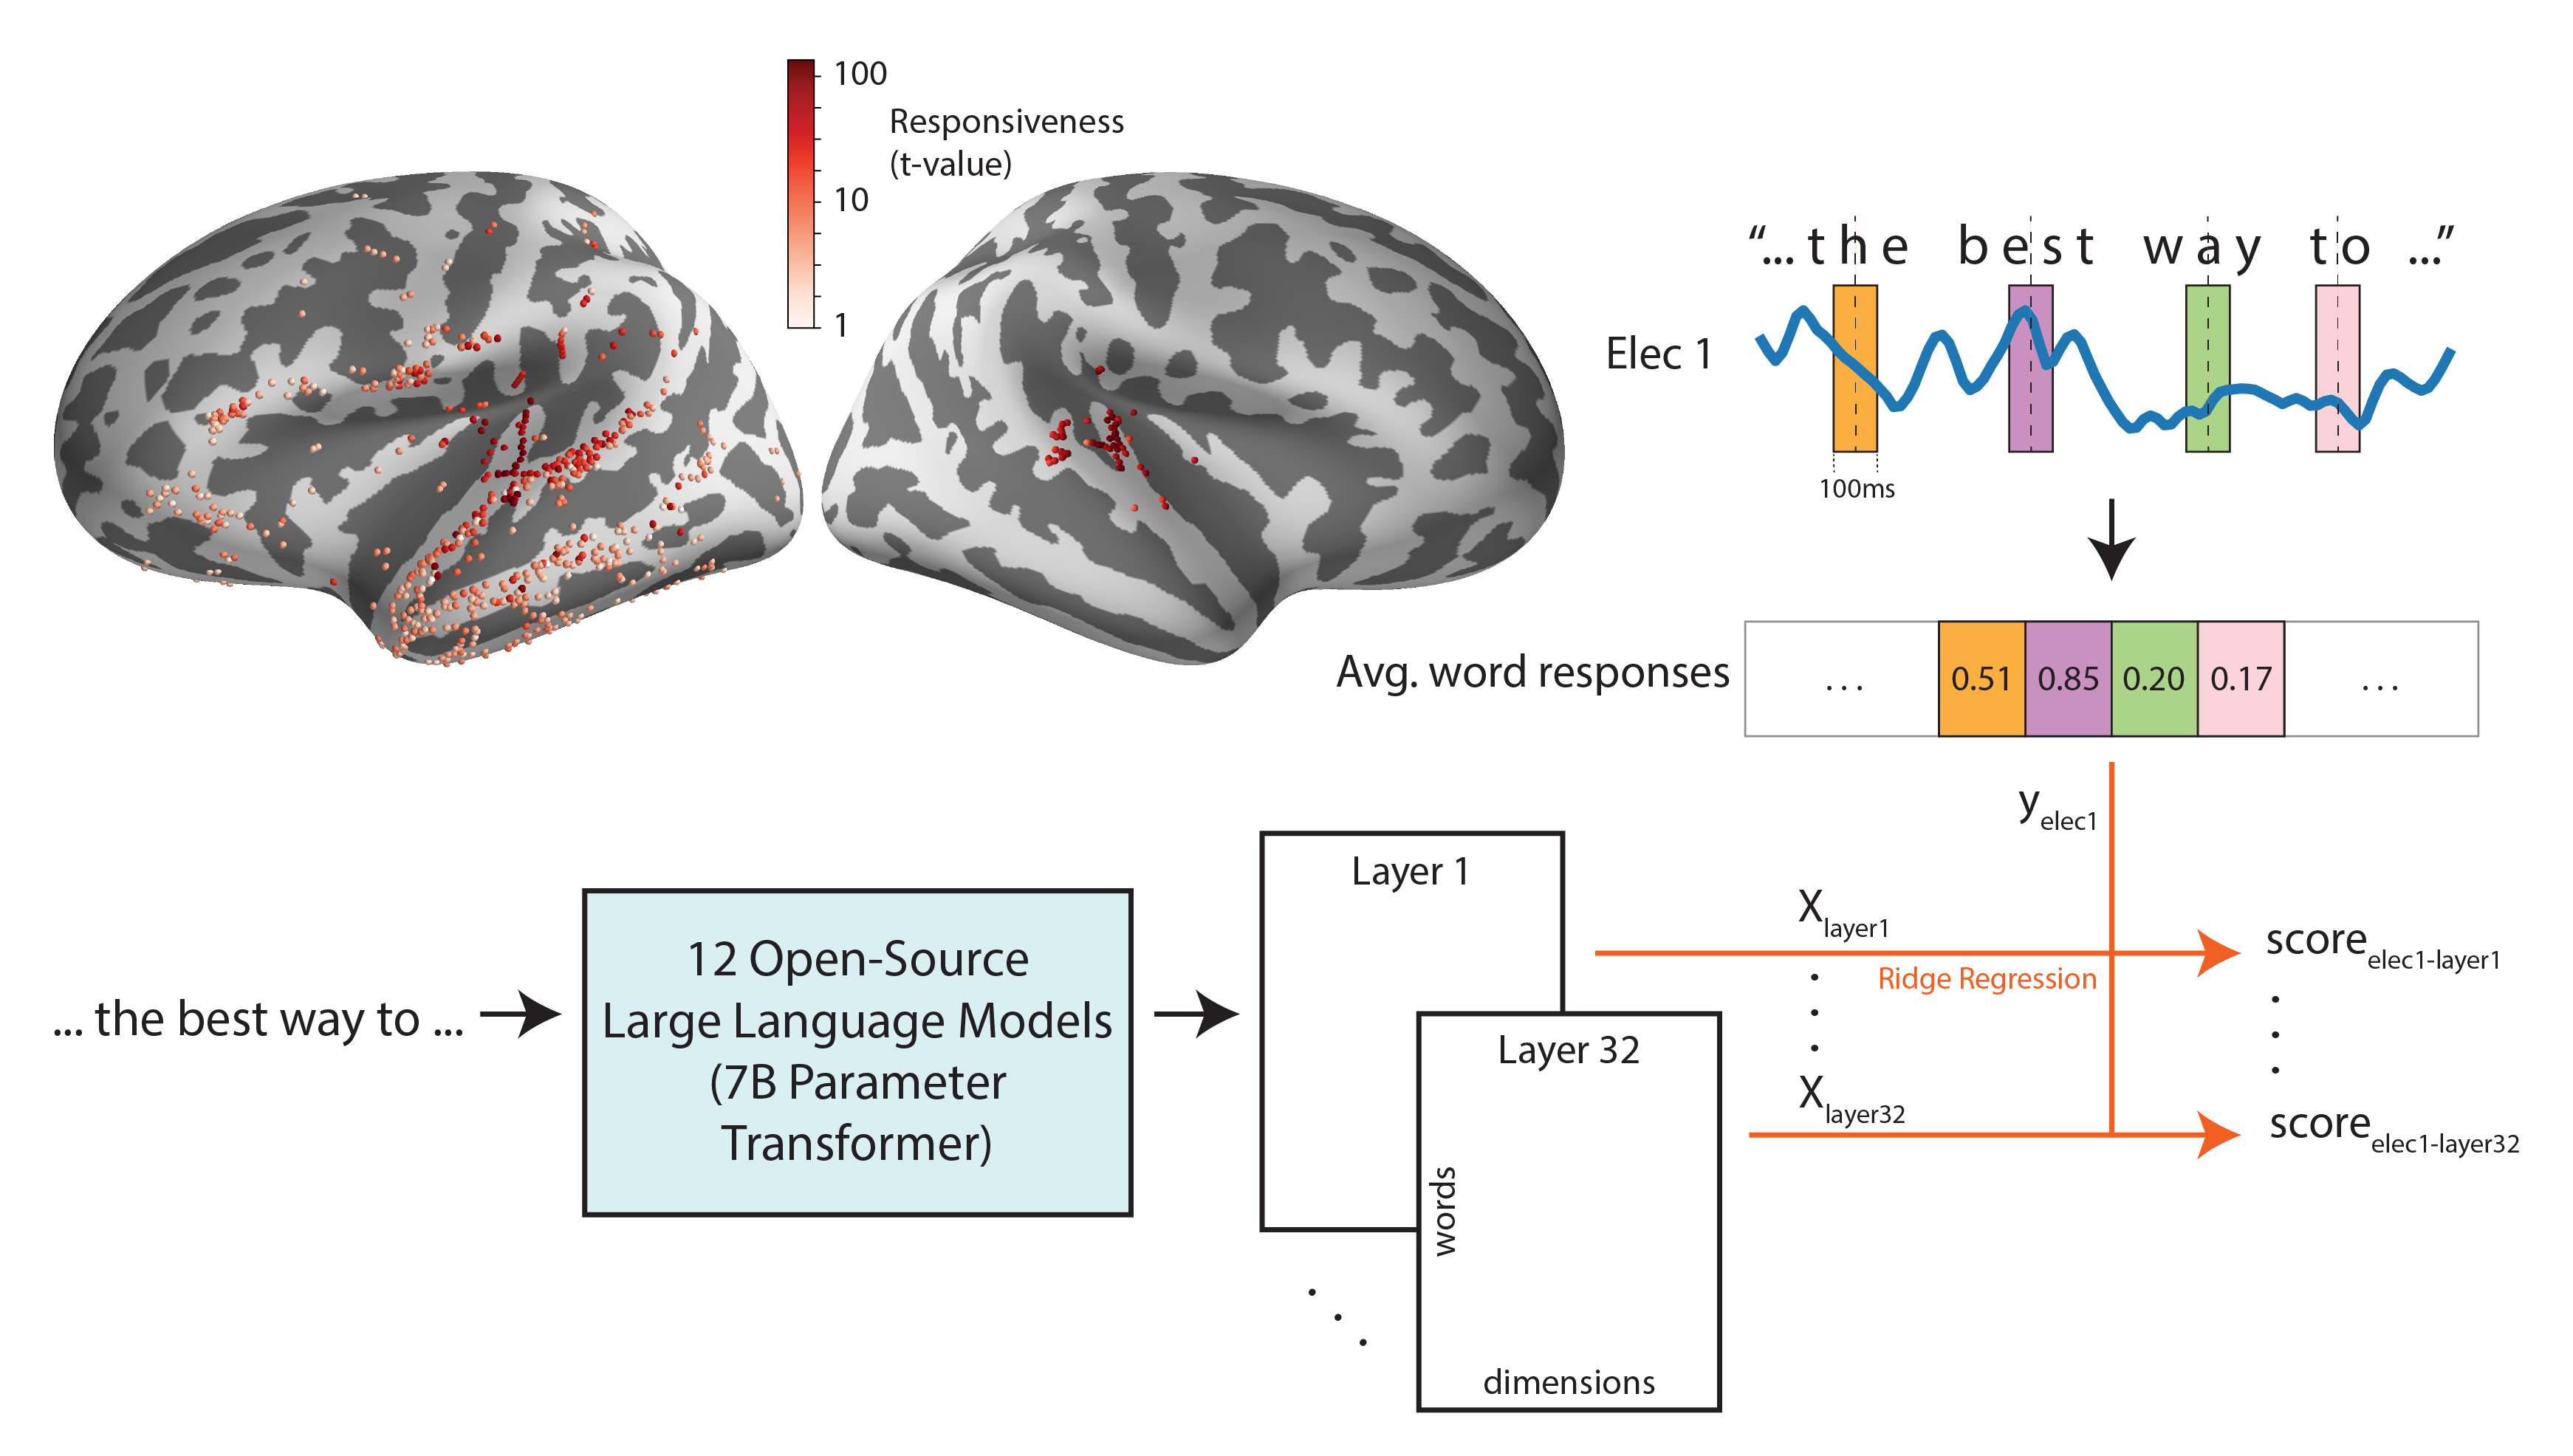
\includegraphics[width=0.95\linewidth]{figures/Figure_regression-illustration2-01.png}}
  \caption{Mapping LLM embeddings to the brain. Speech responsive electrodes are shown on an inflated brain (shaded by their responsiveness t-value from a paired t-test between speech and silence). As subjects listened to speech, the average neural response in a $100$ms window around a word center was used as a given electrode's word response. The same text was fed to an LLM and the embeddings from all $32$ layers were extracted. Ridge regression was used to predict the word responses from the LLM representations, producing a brain correlation score for each electrode-layer pair.}      
  \label{fig:1}
\end{figure}

We studied $12$ recent, popular, open-source LLMs, all with approximately $7$ billion parameters. We evaluated each model on a suite of benchmark tasks to assess its language modeling performance, splitting these tasks into categories relevant to English language comprehension, specifically reading comprehension and commonsense reasoning as in \cite{touvron2023llama2} (see Methods for details). Overall LLM performance was estimated as the average score over these two categories.

\begin{figure}[!t]
  \centering
  % \fbox{\rule[-.5cm]{0cm}{4cm} \rule[-.5cm]{4cm}{0cm}}
  {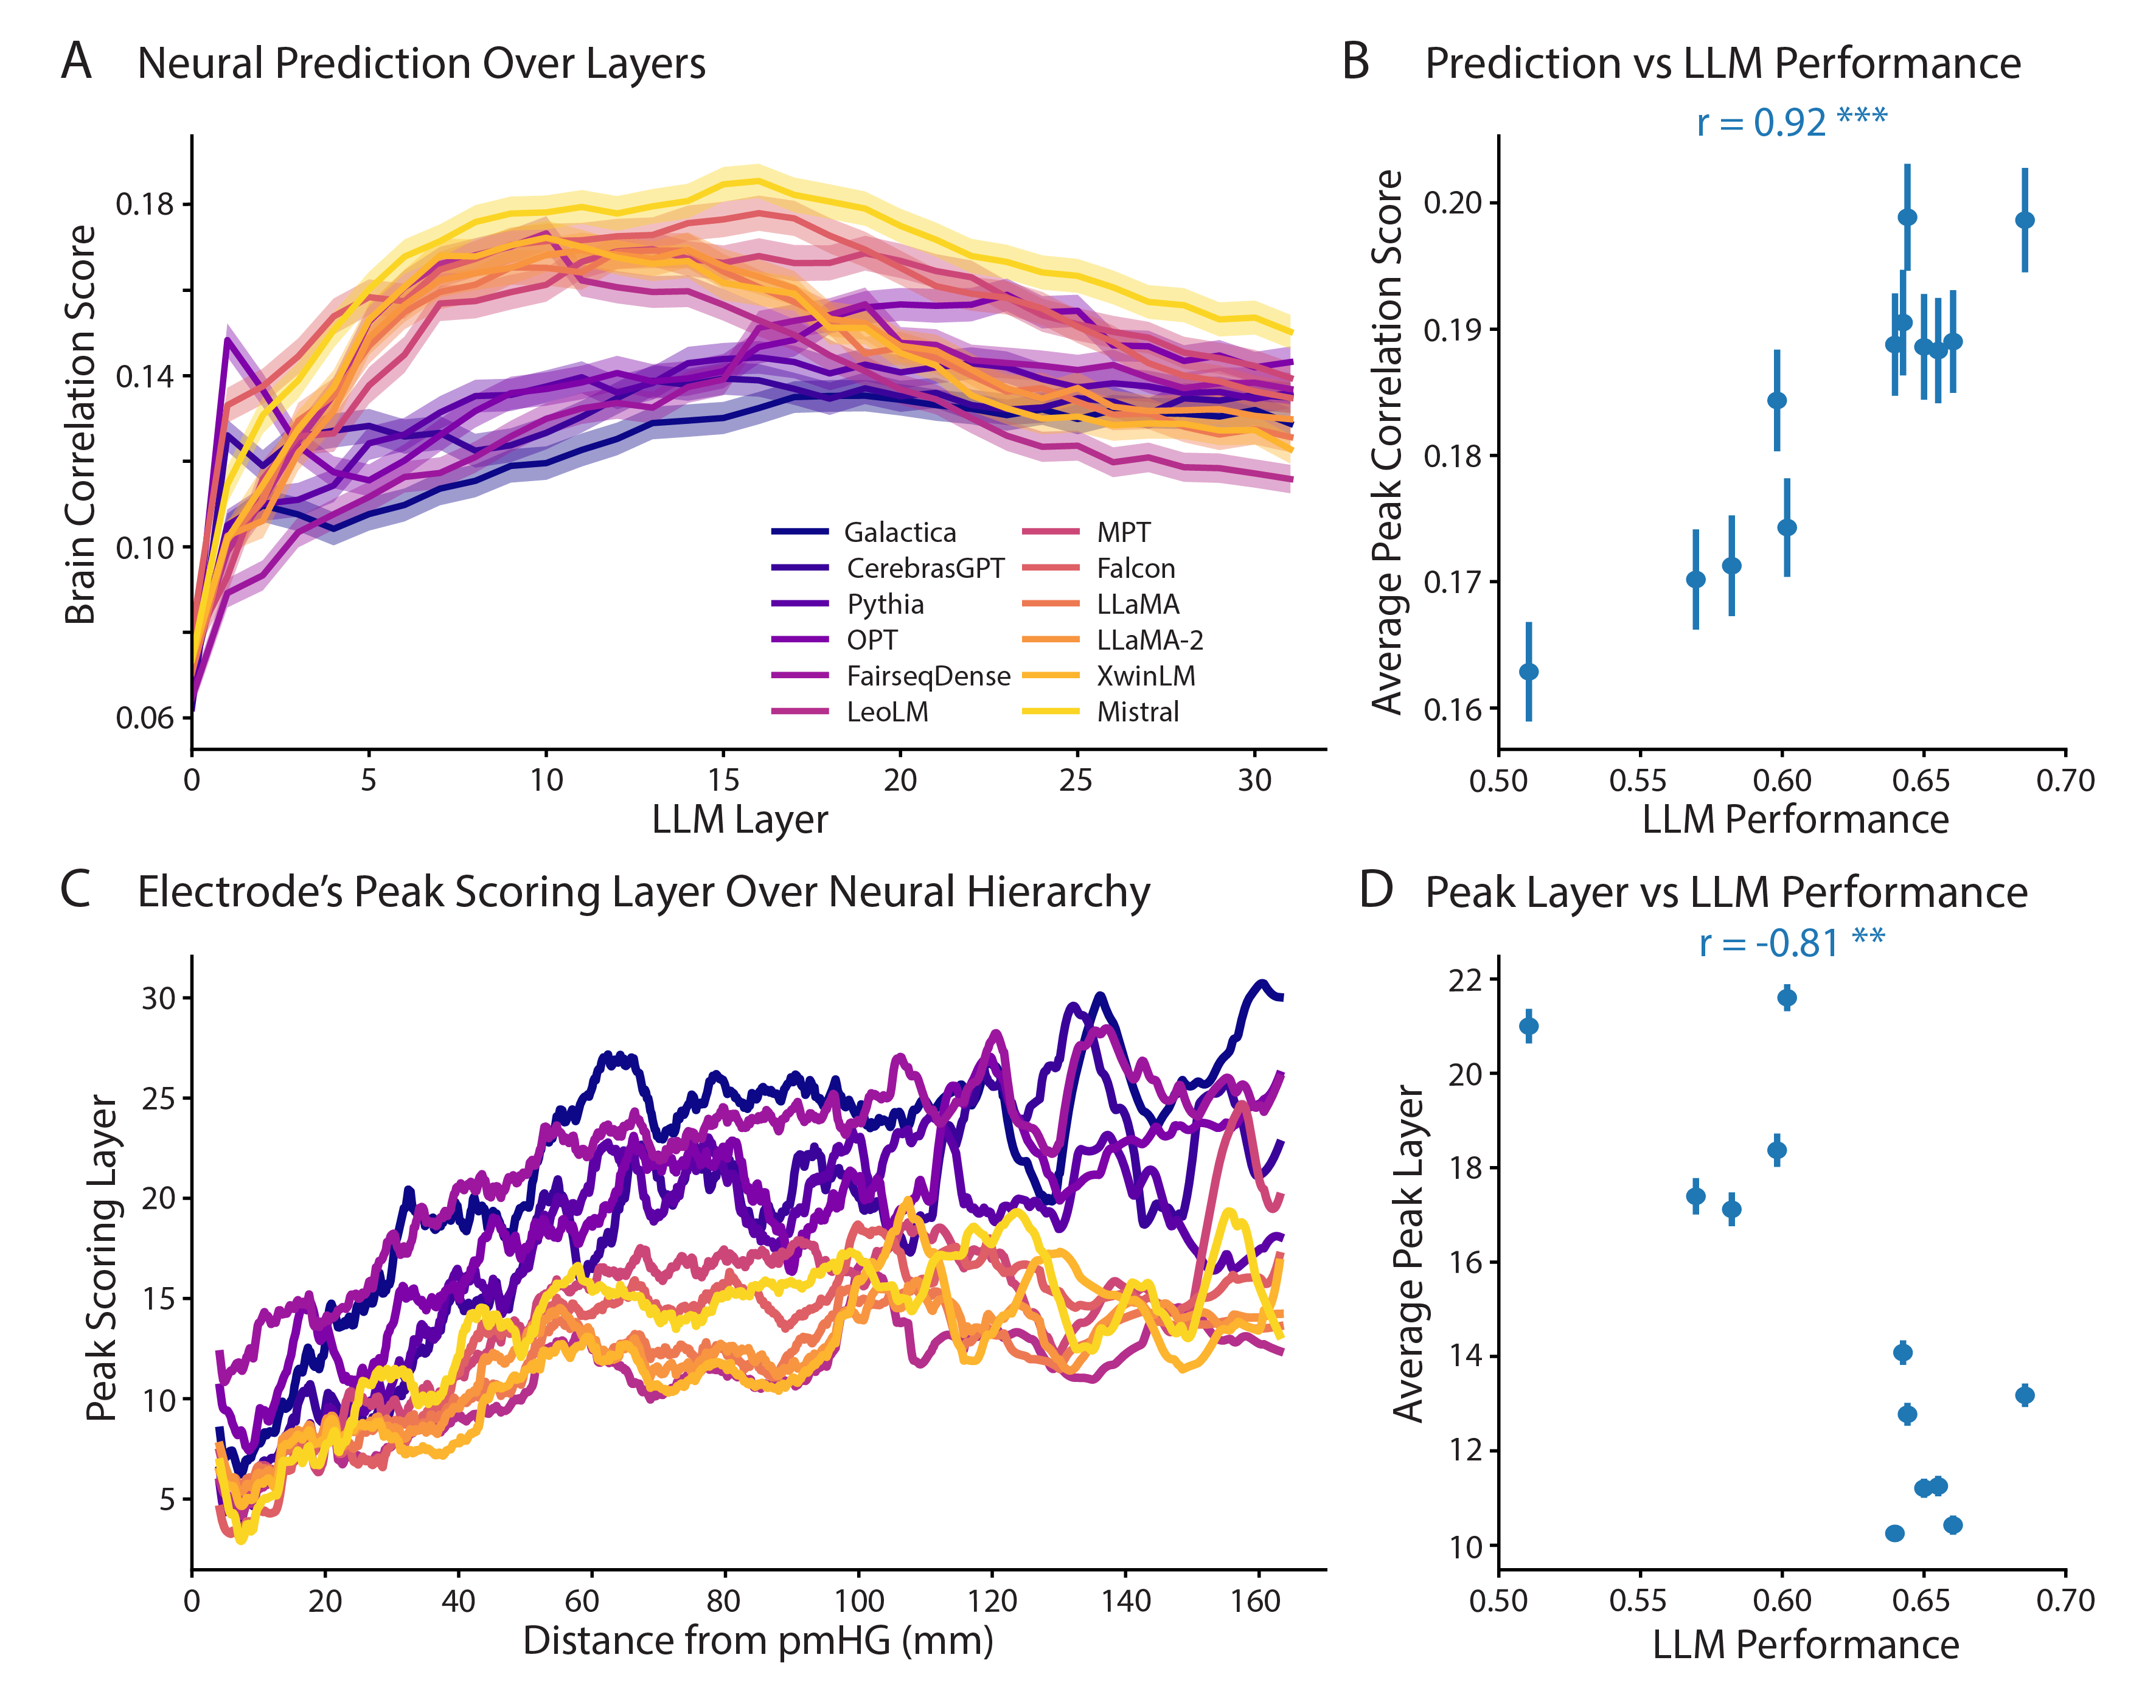
\includegraphics[width=0.95\linewidth]{figures/Figure_peakscores-peaklayers-01.png}}
  \caption{Peak brain correlations and layers relate to LLM performance. A) Average brain correlation over all electrodes for each LLM. LLMs are colored in order of their separately-measured benchmark performance, with blue/purple models performing the worst and yellow models performing the best. Shaded regions indicate standard error of the mean over electrodes. B) The peak correlation over all layers of a given model was computed for each electrode, then averaged over all electrodes. Bars indicate standard error of the mean over electrodes. Average peak correlation score is significantly related to LLM performance (Pearson $r=0.92, p=2.24\times10^{-5}$). Stars indicate statistical significance level thresholds of $p<0.05$, $p<0.01$, and $p<0.001$ with *, **, and ***, respectively. C) The peak scoring layer of each model was computed for each electrode. Then electrodes were sorted by distance from pmHG and a sliding window average (centered, $n=50$) was taken across the electrodes of each model to compute the smoothed, local estimate of the most brain-like LLM layer. The peak scoring layer generally increases with distance from pmHG, and the better models (yellow) peak at lower layers compared to the worse models (blue/purple). D) The average peak layer for a given model over all electrodes is shown with bars indicating standard error of the mean. Average peak layer is significantly negatively related to LLM performance (Pearson $r=-0.81, p=0.0013$).}
  \label{fig:2}
\end{figure}

Neural responses were recorded with invasive electrodes (intracranial EEG) from eight neurosurgical patients, with electrode placement determined by clinical need (Supplementary Fig. 1). The subjects listened to between $20$ and $30$ minutes of speech from various talkers, including stories voiced by voice actors and dialogues between characters. The text for each audio was fed into each LLM, and we extracted the causal embeddings of each word at every layer. We reduced these embeddings to $500$ components with PCA, ensuring consistent dimensionality across models since the models were only approximately the same size to begin with. We used ridge regression to estimate the similarity of a model’s features to the brain (Fig. \ref{fig:1}) \cite{goldstein2022shared, schrimpf2021neural, caucheteux2022brains}. We analyzed $707$ electrodes which were responsive to speech, as determined by a t-test between responses to words and silence (FDR corrected, $p<0.05$ \cite{holm1979simple}). For each responsive electrode, we extracted the average high-gamma band envelope response in a $100$ms window around the center of every word. Then, we fit cross-validated ridge regression models to predict these neural responses from the word embeddings and used the average prediction correlation on the withheld folds as the brain similarity with that electrode. Neither the number of principal components of the embeddings nor the window size used to compute the neural response to words significantly impacted the results (Supplementary Fig. 2).


Electrode-averaged brain similarity over each model's layers is shown in Fig. \ref{fig:2}A. With these latest LLMs, we confirm previous findings showing that neural responses can be predicted from model representations, and we find that brain similarity generally increases over layers and peaks in middle or later layers \cite{schrimpf2021neural, caucheteux2022brains}. Higher-performing LLMs also achieve higher peak brain scores (Pearson $r=0.92, p=2.24\times10^{-5}$) (Fig. \ref{fig:2}B), indicating that they extract more brain-like features from language.

Similar to the layers of a model, the auditory and language processing pathway demonstrates hierarchical organization \cite{hickok2007cortical, sharpee2011hierarchical, hasson2008hierarchy, lerner2011topographic}. The primary auditory cortex, the first point of auditory processing in the cortex, is centered around posteromedial Heschl’s gyrus (pmHG, or TE1.1) \cite{morosan2001human}. Since this is a common reference point in auditory cortical processing, we quantify the depth of each electrode in the brain’s spoken language processing pathway using its distance from this landmark \cite{baumann2013unified, norman2018neural, mischler2023deep}. Prior studies have found that deeper layers of LLMs correspond better to deeper language processing regions of the brain \cite{caucheteux2022brains, caucheteux2023evidence, kumar2022reconstructing}. We confirm this result (Fig. \ref{fig:2}C), but interestingly, we also find that better-performing LLMs peak in brain similarity at earlier layers compared to worse models (Pearson $r=-0.81, p=0.0013$) (Fig. \ref{fig:2}D). This uncovers a new dimension in the evolution of LLMs: the progression of feature extraction over layers aligns differently with the brain for higher-performing versus lower-performing models.


\subsection{Alignment of Language Processing Hierarchies Between Models and the Brain}

\begin{figure}[!t]
  \centering
  % \fbox{\rule[-.5cm]{0cm}{4cm} \rule[-.5cm]{4cm}{0cm}}
  {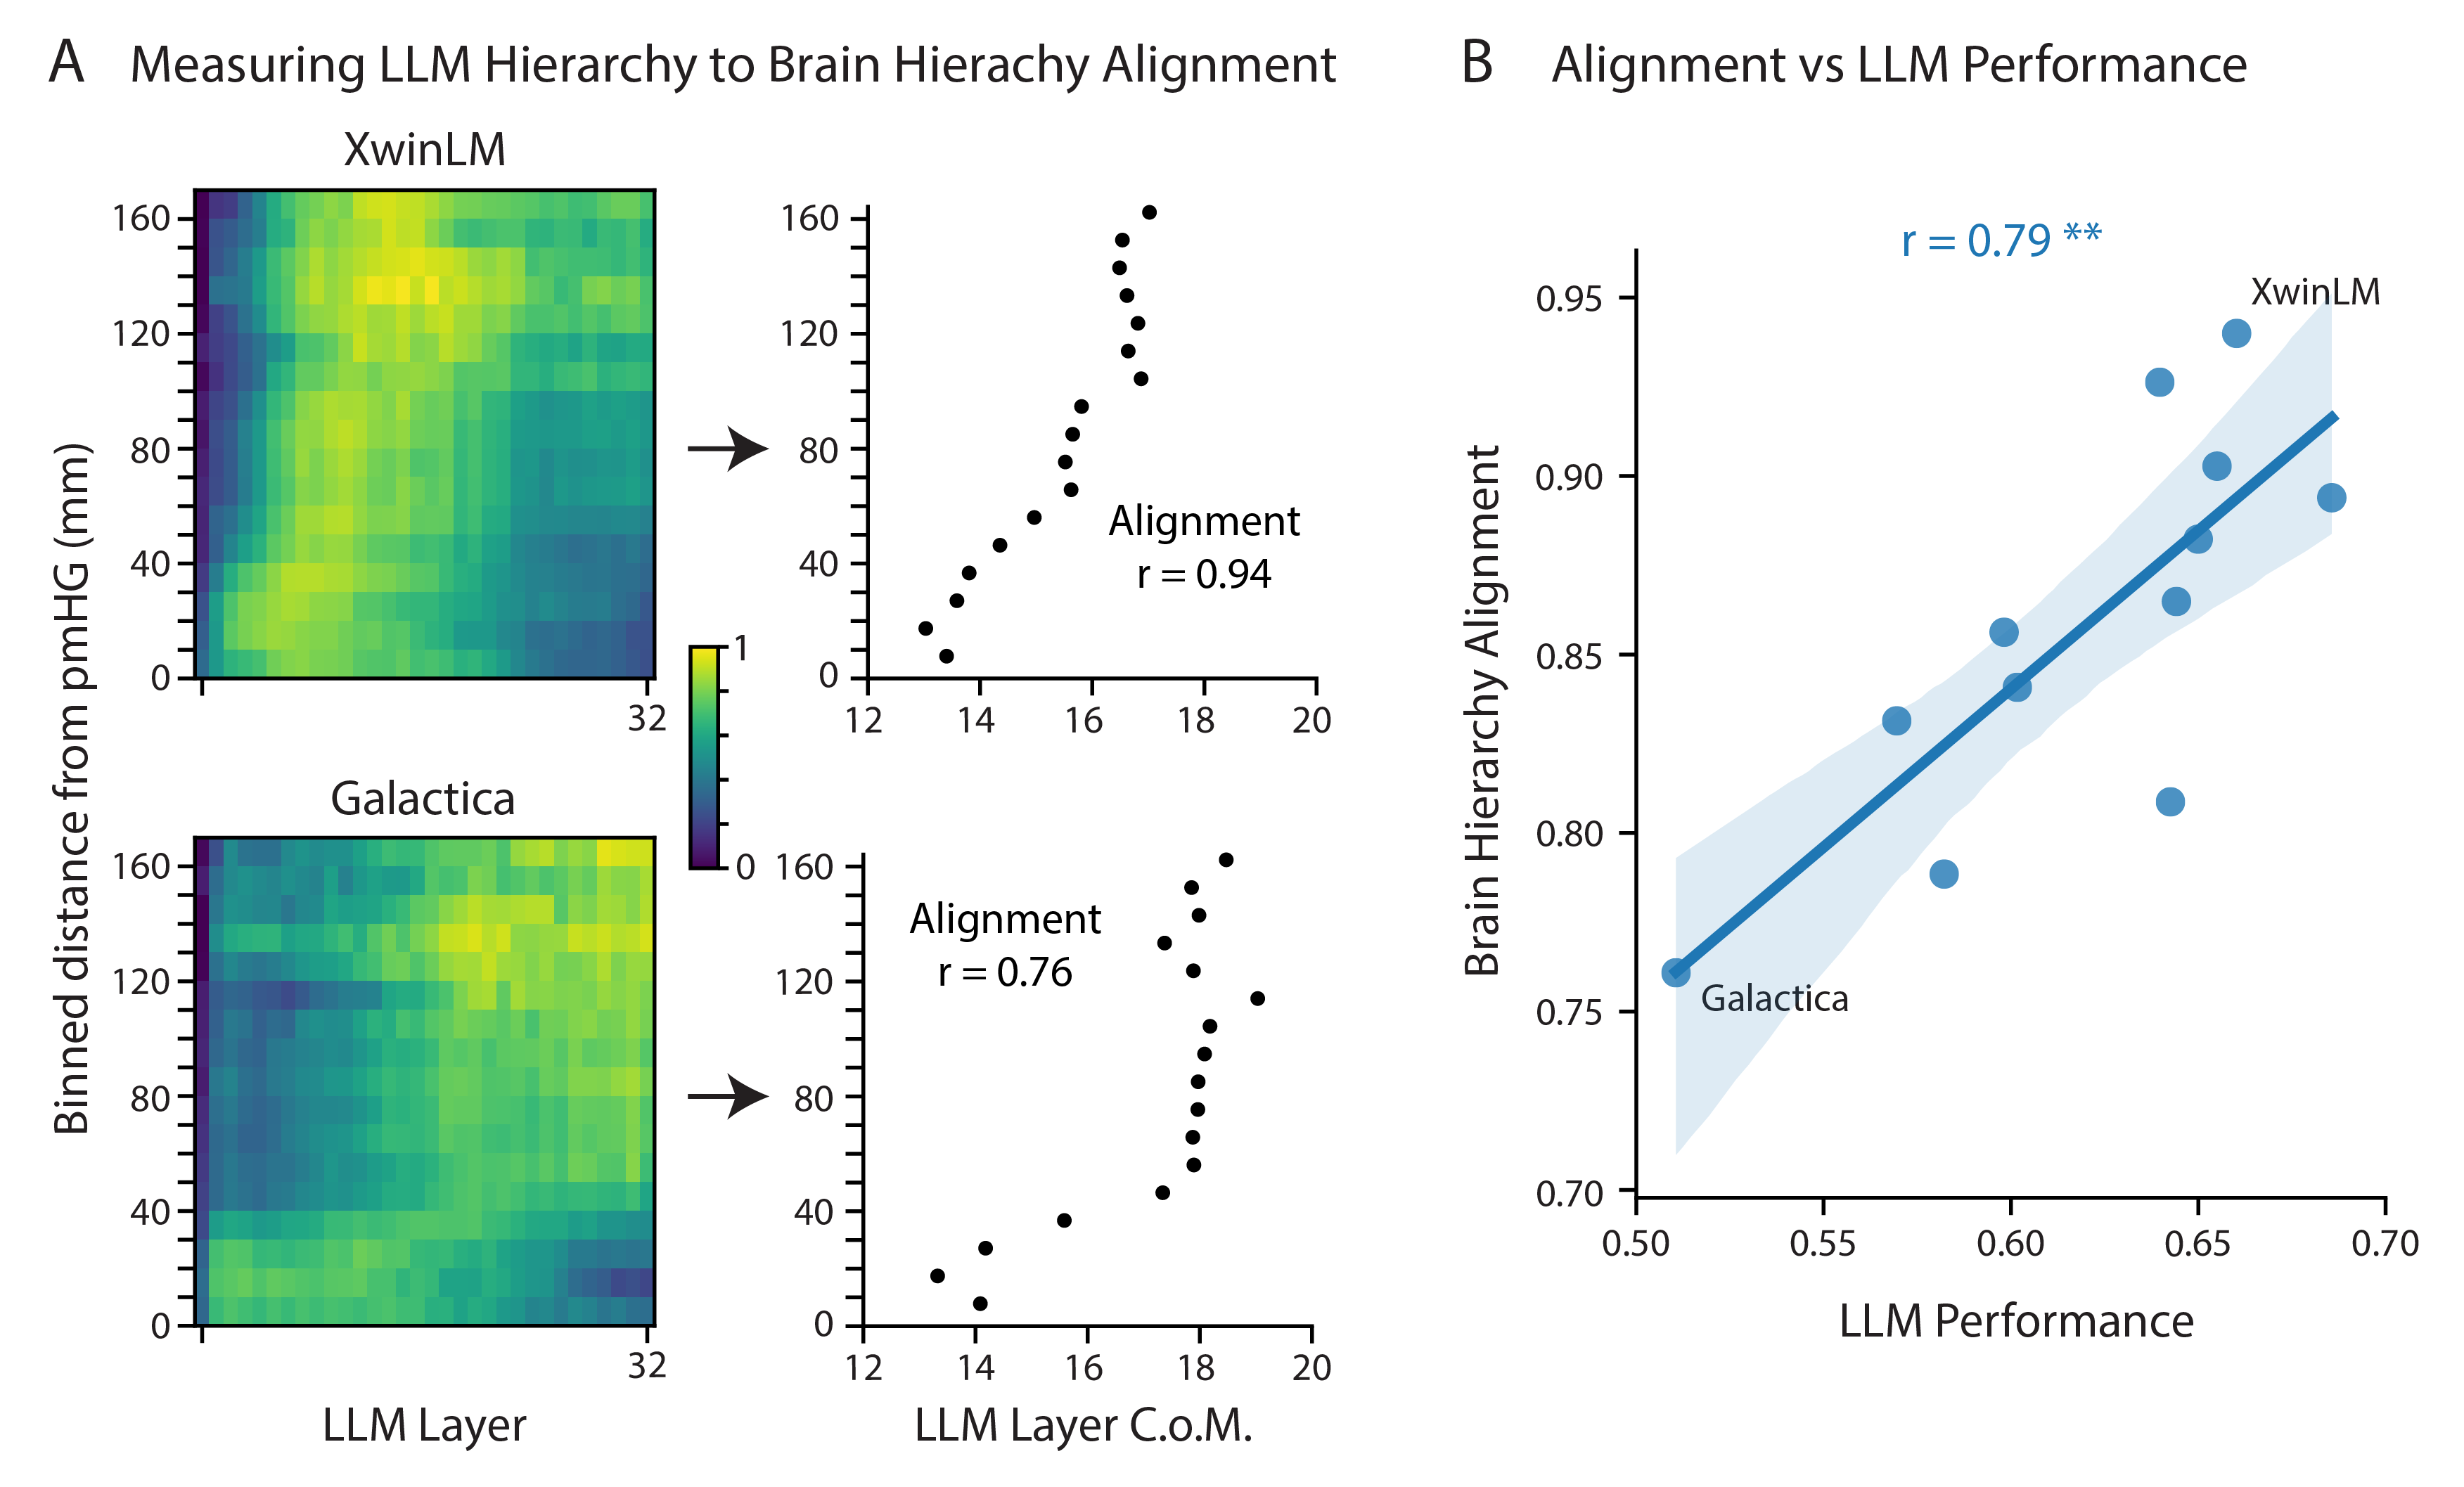
\includegraphics[width=0.95\linewidth]{figures/Figure_brain-model-alignment-method-distance-01.png}}
  \caption{Better LLMs display more brain-like hierarchical processing. A) Examples of computing the brain hierarchy alignment are shown for two models: XwinLM (the model with the highest alignment score) and Galactica (the model with the lowest alignment score). Electrodes were first binned into a hierarchy by distance from pmHG. Within a bin, the correlations over all 32 layers were normalized between 0 and 1 and then averaged over electrodes in the bin, producing one row for each bin in the matrix on the left. The center of mass (C.o.M.) of the distribution of brain similarity scores over LLM layers for each bin was computed and plotted in the scatter plot to the right. The brain hierarchy alignment score was then computed as the Pearson correlation between LLM layer C.o.M. and distance from pmHG. B) A scatter plot of brain hierarchy alignment scores and LLM performance shows a significant positive correlation (Pearson $r=0.79, p=0.0021$, ** indicates $p<0.01$). Line and shaded region shows linear regression fit and bootstrapped $(n=1000)$ $95\%$ confidence interval.}
  \label{fig:3}
\end{figure}

Given that the layer-wise brain similarity appears different between good and bad models, we hypothesized that better models were not only learning more brain-like features, but that the progression of feature extraction within these models was different. Taking inspiration from an investigation of hierarchical correspondence between stages of visual cortex processing and image classification networks \cite{nonaka2021brain}, we sought to compute the alignment between hierarchical feature extraction pathways in brains and models. Although the brain's exact hierarchical processing stages, analogous to layers of a model, are not perfectly known, we again used the distance from pmHG to quantify the stages of hierarchical processing. We grouped electrodes into bins at 10mm intervals. Then, for each electrode, we normalized the brain similarity scores over layers. Finally, we averaged these layer-wise scores over the electrodes in a bin, producing a set of layer scores which are shown as a single row of the alignment matrix in Fig. \ref{fig:3}A. We used the center of mass of this average brain similarity score over layers within each electrode bin to quantify the LLM layer most similar to a given stage of the brain's hierarchy. Then, we compared the progression of these most-similar LLM layers to the bin distances along the hierarchy, visually finding that some models achieve a more linear increase in LLM layers over bins. We summarize the alignment between the language processing hierarchies of each LLM and the brain using the Pearson correlation between the layer center of mass in each bin and the hierarchical stage of each bin (i.e. the distance of each bin from pmHG) \cite{nonaka2021brain}. We illustrate this alignment computation for XwinLM and Galactica, two models which achieve the highest and lowest hierarchy alignment scores, respectively (Fig. \ref{fig:3}A). These models also display a stark difference in benchmark performance, with Galactica being the lowest performing LLM. The alignment scores reveal that the better model (XwinLM) exhibits a feature extraction progression more consistent with the brain from early to late-stage processing compared to the bad model.  This brain alignment is also highly correlated with LLM performance on the benchmark evaluation tasks (Pearson $r=0.79, p=0.0021$) (Fig. \ref{fig:3}B). We find the same result when using electrode latency to measure the stages of the brain's hierarchical processing, rather than distance from pmHG (Pearson $r=0.89, p=0.0001$) (Supplementary Fig. 3), which demonstrates that this finding holds for other estimates of the stages of the cortical hierarchy. Additionally, to ensure this effect was not the result of a single subject overpowering the distribution, we separated the even- and odd-numbered subjects and performed the analysis again, finding that brain hierarchy alignment was significantly correlated with LLM performance for each group (Pearson correlation, even subjects: $r=0.79, p=0.0022$, odd subjects: $r=0.81, p=0.0013$) (Supplementary Fig. 4). Overall, these findings demonstrate that better-performing LLMs extract features using a hierarchy that more linearly aligns with the brain's hierarchical language processing pathway.

\begin{figure}[!t]
  \centering
  % \fbox{\rule[-.5cm]{0cm}{4cm} \rule[-.5cm]{4cm}{0cm}}
  {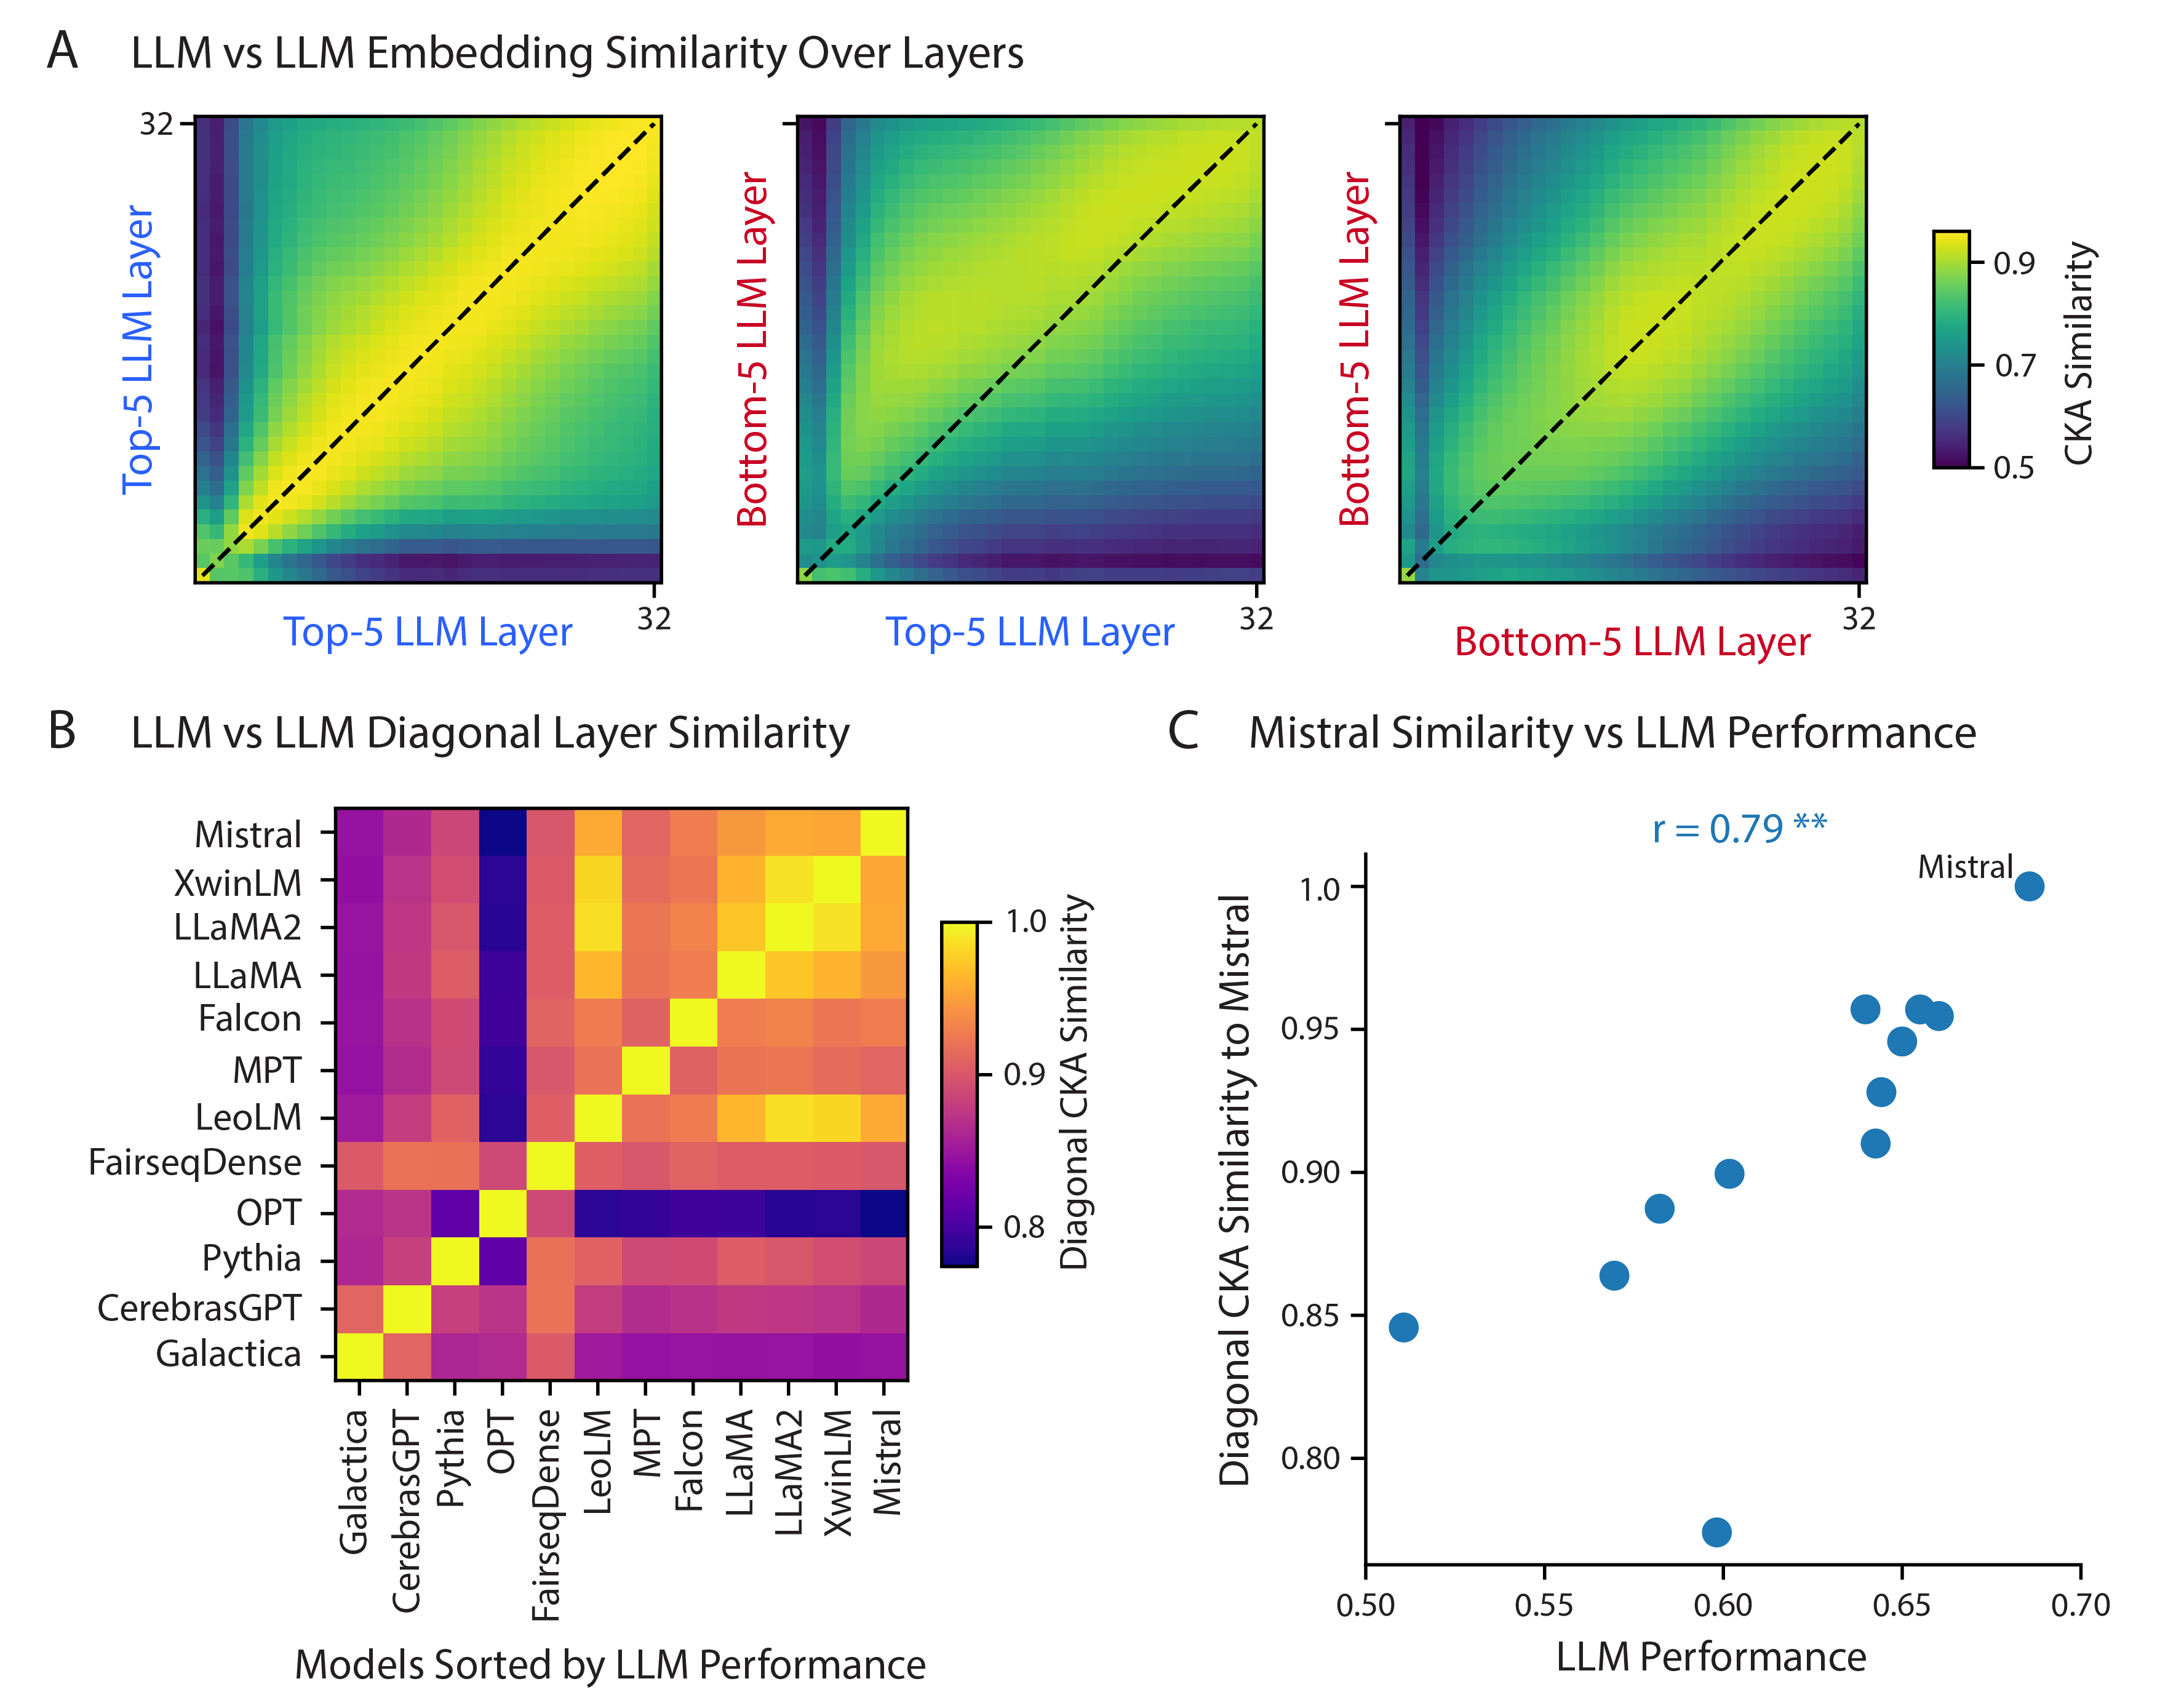
\includegraphics[width=0.95\linewidth]{figures/Figure_good-vs-bad-vs-good-imshow-1x3plots-01.png}}
  \caption{Comparing feature extraction hierarchies between LLMs. A) Layer-by-layer similarity matrices were computed using CKA for every pair of LLMs. LLMs were labeled as either top-5, bottom-5, or excluded, depending on their sorted performance on our LLM benchmark evaluation. Then, similarity matrices between all pairs of top-5 LLMs were averaged and displayed as the ``top-5 versus top-5'' average similarity matrix in the top left. The same was done to create similarity matrices between the average ``top-5 versus bottom-5'' as well as the average ``bottom-5 versus bottom-5'' LLMs. Visually, the ``top-5 versus top-5'' similarity matrix is highly diagonal, while ``bottom-5 versus bottom-5'' is less similar in early layers. The ``top-5 versus bottom-5'' similarity matrix shows an offset diagonal, indicating a delay in feature extraction for the bottom-5 models compared to the top-5. B) Model-by-model diagonal similarity was computed as the average along the diagonal of their similarity matrix. Models are arranged in sorted order of LLM benchmark performance from worst to best. This visually confirms that the best models are fairly similar to each other in layer-wise feature extraction, while worse models are less similar to each other and less similar to the best models. C) The diagonal similarity of each model with Mistral, the best performing LLM, is plotted against the LLM performance, showing a strong positive relationship (Pearson $r=0.79, p=0.0022$, ** indicates $p<0.01$).}
  \label{fig:4}
\end{figure}

To perform model-to-model comparisons, we used centered kernel alignment (CKA) \cite{kornblith2019similarity}, a method analogous to canonical correlation analysis (CCA) with a nonlinear kernel, which is able to capture similarity between high-dimensional representations like neural network embeddings. We computed the CKA similarity between all pairs of layers for all pairs of models. Thus, each pair of models creates a layer-by-layer similarity matrix describing their embedding similarity. High similarity along the diagonal indicates that the two models extract similar features at the same layers. Higher similarity offset from the diagonal indicates that one model exhibits a delay in extracting similar features. When grouping these similarity matrices by the top-5 and bottom-5 models based on LLM benchmark performance and averaging within a group, an interesting pattern emerges (Fig. \ref{fig:4}A). We find that the top models exhibit a high degree of similarity to each other along the diagonal. On the other hand, the worst models are much less similar to each other in their early layers, and even in their later layers they are less consistent than the top-5-to-top-5 model pairs. Finally, comparing top-5 models to bottom-5 models reveals a striking offset in maximum similarity from the diagonal. This suggests that bad models require more layers to reach a similar level of feature extraction as good models. We summarize the layer-wise feature extraction similarity between each pair of models using the average CKA similarity along the diagonal in their CKA similarity matrix (Fig. \ref{fig:4}B). The plot demonstrates that the top-5 models are indeed more similar to each other, with a sub-block of high similarity emerging among the top few models. Since Mistral is the best performing LLM, we look at the diagonal similarity to Mistral of each model and find that a more Mistral-like feature extraction progression correlates strongly with LLM performance (Pearson $r = 0.79, p=0.0022$) (Fig. \ref{fig:4}C). These results reveal new distinctions between the embeddings of LLMs and suggest that inefficient feature extraction or poor early-layer learning in bad models may contribute to their worse performance and lower brain similarity.


\subsection{Contextual Content Supports Brain Hierarchy Alignment}

Since the contextual nature of LLM features is critical for their brain similarity compared with non-contextual representations \cite{goldstein2022shared, schrimpf2021neural, caucheteux2022deep}, we hypothesized that the amount of contextual information used by a model may also play a key role in determining the alignment between hierarchical feature extraction pathways of LLMs and the brain. We extracted limited-context embeddings from the LLMs by restricting their causal attention mechanism to a certain window of the previous text. Transformer architecture LLMs use tokenizers to separate text into discrete units, so we supplied the models with only the most recent $N$ tokens, sweeping $N$ over a range of values from $1$ to $100$. A single token input gives the model no context at all. For reference, Mistral's tokenizer averages $1.15$ tokens per word in our stimulus corpus. We then repeated our analysis of model-brain hierarchical alignment (as previously shown in Fig \ref{fig:3}B) by computing the correlation between brain hierarchy alignment and LLM performance at each limited context window length. While this correlation is positive for all but the $1$-token case, it is only significant for long contextual window lengths of $50$ tokens and above (Fig. \ref{fig:5}A). This suggests that the brain alignment of LLMs critically depends on the amount of contextual information the model is able to see, which then influences its hierarchical feature extraction mechanism.

\begin{figure}[!t]
  \centering
  % \fbox{\rule[-.5cm]{0cm}{4cm} \rule[-.5cm]{4cm}{0cm}}
  {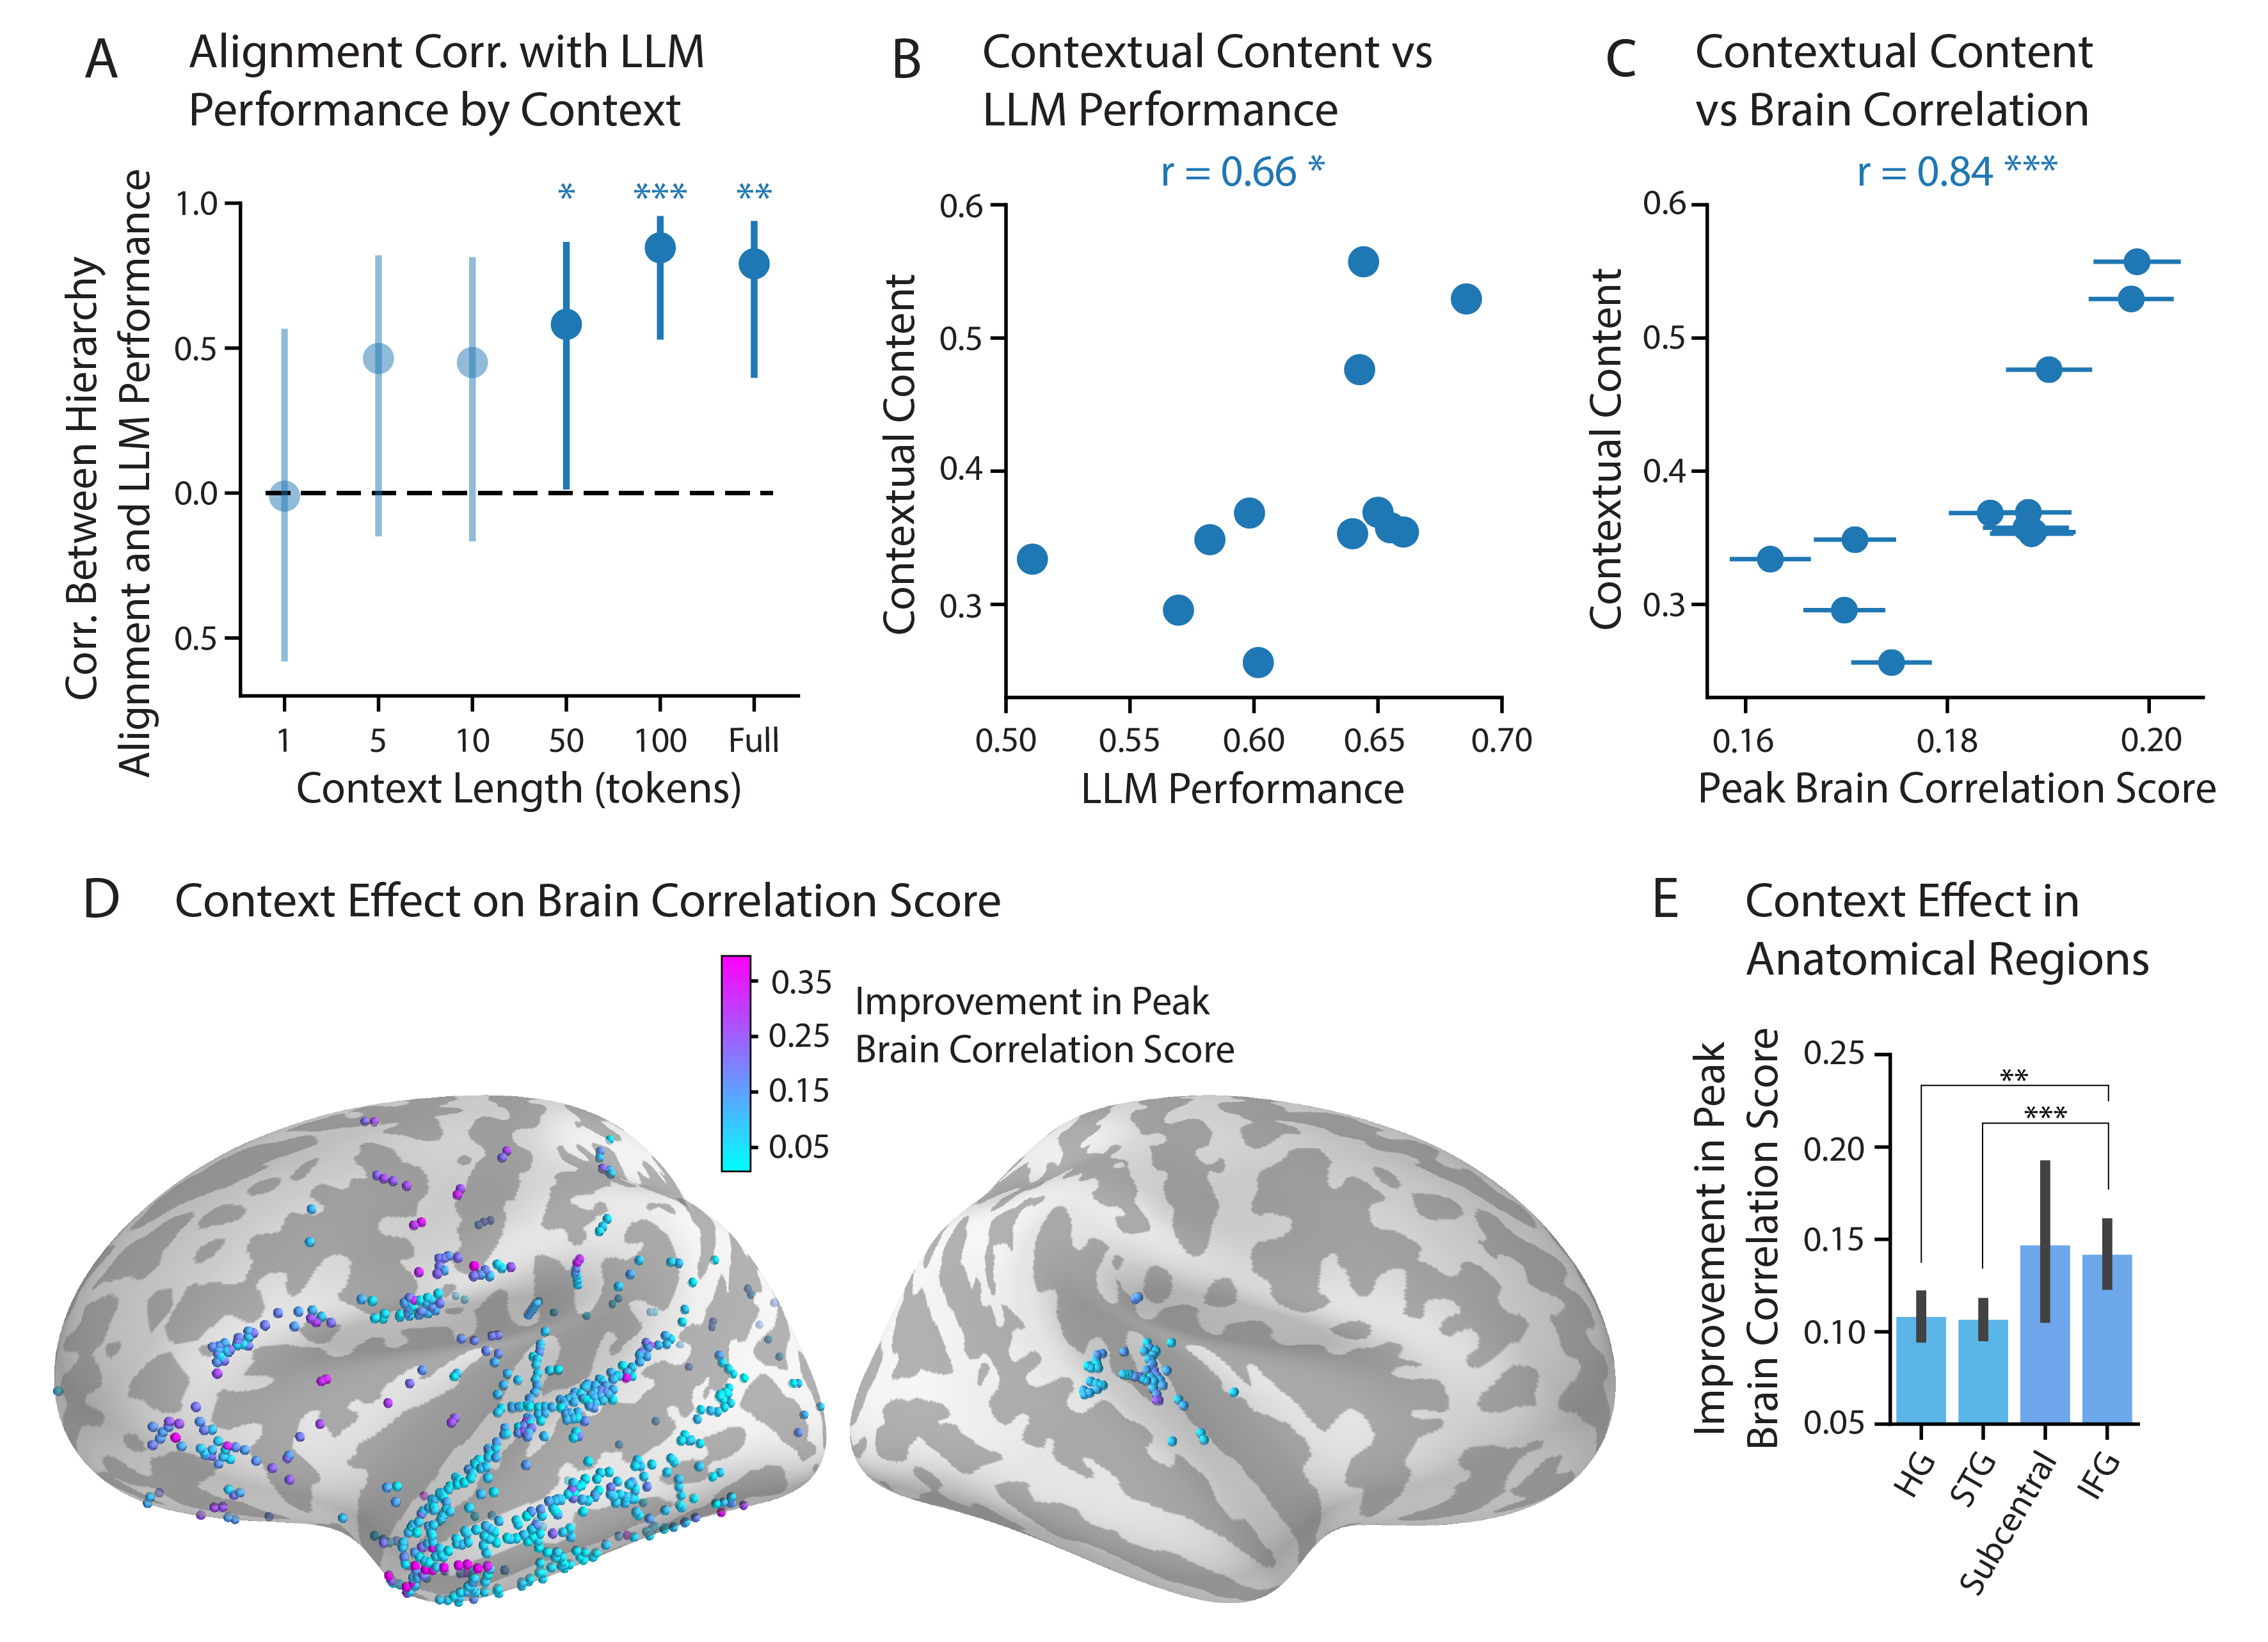
\includegraphics[width=0.95\linewidth]{figures/Figure_context_effects_expandedBrain-01.png}}
  \caption{Effect of contextual information. A) Using embeddings from the LLMs when given a certain limited number of the previous tokens as a context window, we performed the analysis of brain hierarchy alignment again. The correlation between LLM performance and brain hierarchy alignment is illustrated by each dot with 95\% confidence interval bars, showing only a significant correlation for long contextual windows. Stars illustrate the significance level of the correlation, with $*$, $**$, and $***$ indicating chance levels below $0.05$, $0.01$, and $0.001$, respectively. B) The contextual content of a model's representations is plotted against its benchmark performance, showing a positive correlation between the two (Spearman $r=0.66, p=0.020$). C) Contextual content of each model is plotted against its average peak brain similarity over electrodes, showing a strong correlation (Spearman $r=0.84, p=0.0006$). Horizontal lines show standard error of the mean over electrodes for brain similarity. D) Electrodes plotted on the FreeSurfer average inflated brain, colored by the effect of contextual information on peak brain similarity score. E) Bar plot of the average context effect on peak brain similarity score for electrodes within four main anatomical regions along the linguistic hierarchy. Each bar is colored by its value according to the same colormap as used on the brain plot, and error bars show standard error of the mean. Stars indicate significant differences between a pair of regions (Wilcoxon rank-sum test).}
  \label{fig:5}
\end{figure}

Since the correlation between LLM performance and hierarchical alignment is strongly positive for long context lengths, we expected that better-performing models would be better at incorporating contextual information into their language representations. To test this, we quantified the amount of contextual information present in a model's embeddings by measuring how much its embeddings changed when contextual information was added to the input. We measured the CKA difference ($1 - \text{similarity}_{CKA}(\text{full-context}, \text{1-token})$) of the embeddings of each layer when given the full context compared to the first-layer embeddings when given only a $1$-token limited context window. We refer to the average of this CKA difference over all layers as the contextual content of the model's representations. We find that this contextual content is positively correlated with LLM performance (Spearman $r=0.66, p=0.020$) (Fig. \ref{fig:5}B). Additionally, it is very strongly correlated with brain similarity (Spearman $r=0.84, p=0.0006$) (Fig. \ref{fig:5}C). These findings indicate that contextual information plays a crucial role in natural language processing in both natural and artificial language models, and contextual feature extraction enables brain hierarchy alignment in LLMs.

%% either figure
We further investigated the impact of contextual information on neural similarity by computing how much each LLM's peak similarity score with a given electrode changed when the models were given the full context versus no context ($1$ token). 
% if og figure
% Averaging this difference over all LLMs for each electrode, we find that peak brain similarity scores improve more for electrodes further from pmHG (Pearson $r=0.093, p=0.012$) (Fig. \ref{fig:5}D).
% if new figure
We then averaged this difference over all LLMs for each electrode and plotted the electrodes on the brain, finding that being given the extra context more greatly improved similarity scores with electrodes in higher-level language processing areas (Fig. \ref{fig:5}D). Averaging electrodes within major anatomical regions further quantifies this result, as we find higher average context effects on brain correlation score within the higher-level linguistic-processing area of inferior frontal gyrus (IFG) \cite{costafreda2006systematic} compared to sensory regions like Heschl's gyrus (HG) and superior temporal gyrus (STG) (Wilcoxon rank-sum test, $p<0.05$) (Fig. \ref{fig:5}E). Interestingly, the articulatory region of subcentral gyrus, which has also been implicated in high-level linguistic processing \cite{arana2020sensory}, displays the highest average score improvement, but due to its high variance it does not meet statistical significance.
% either figure
These results show that contextual information becomes more critical in determining brain similarity further along the spoken language processing hierarchy, which supports previous investigations of high-level linguistic feature encoding in more downstream regions \cite{sheng2019cortical, keshishian2023joint}. 
% if og figure
% This is also visible in a brain plot (Fig. \ref{fig:5}E). Averaging electrodes within major anatomical regions further quantifies this result, as we find higher average context effects on brain correlation score within the higher-level linguistic-processing area of inferior frontal gyrus (IFG) \cite{costafreda2006systematic} and the articulatory region of subcentral gyrus which has also been implicated in high-level linguistic processing \cite{arana2020sensory} compared to sensory regions like Heschl's gyrus (HG) and superior temporal gyrus (STG) (Fig. \ref{fig:5}E). 
%% either figure
This finding strengthens the notion that both the brain and LLMs are extracting context along their hierarchies, and that LLMs need contextual information to achieve brain similarity in downstream processing regions. Taken together, our analyses reveal that high-performing LLMs not only extract representations of language that are similar to the brain, but they also use hierarchical feature extraction pathways which more strongly align with that of the brain due to contextual information processing abilities, a finding that uncovers new ways in which the best LLMs are continuously converging toward the brain.
